\section{Suggestive Interface for Shape Modification }\label{sec:interaction}
%
For some creative designs, the rough 3D carton model generated based on our heuristic approach still needs some improvements or the user might edit the carton shape. 
%After folding the flat layout into a rough shape, we need to refine the model to final state through basic geometric constraints and user-selected constraints which are obtained from user interaction. 
To help common users refine the carton model, our system is equipped with a set of smart shape refinement operations, such as automatically detecting vertexes that can be merged, propagating modifications to similar groups, and providing suggestions for users to explore. 
%
Moreover, when the user edits a carton model in the 3D space, which is more intuitive, our system is capable of revising the 2D layout automatically. 

 
\subsection{Suggestive Interaction}

Our system automatically detects a group of potential shape constraints to improve the 3D carton model. 
These guiding constraints are provided to the user for to quickly select and manipulate the carton shape.
In our system, three types of shape refinement operations, vertex merging, merging propagation, and face pasting, are automatically detected.


\begin{figure}
	\centering
	\subfigure[Vertex Merging]{
		\label{fig:suggestion:a} %% label for first subfigure
		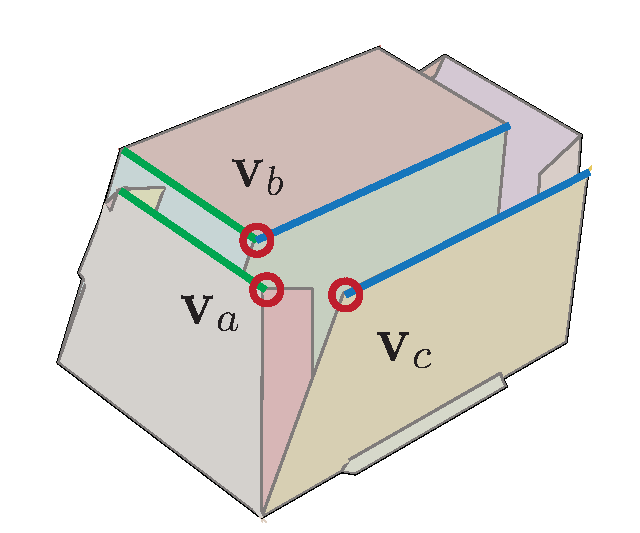
\includegraphics[width=0.25\textwidth]{images/suggestiona.pdf}}
	\hfill
	\subfigure[Merging Propagation]{
		\label{fig:suggestion:b} %% label for second subfigure
		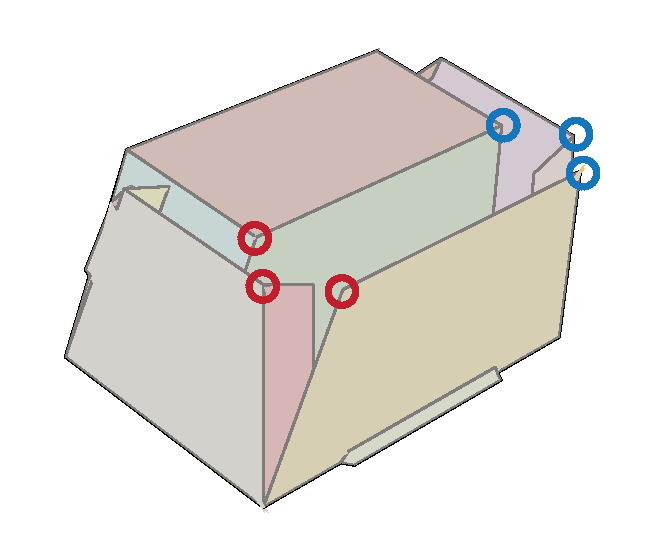
\includegraphics[width=0.25\textwidth]{images/suggestionb.pdf}}
	\hfill
	\subfigure[{Panel Pasting}]{
		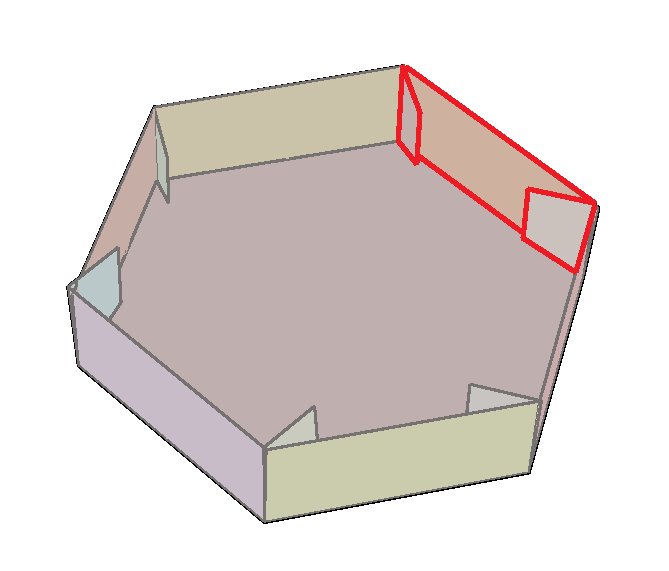
\includegraphics[width=0.25\textwidth]{images/suggestionc.pdf}
		\label{fig:facepasting}
	}
	
	\caption{Three different suggestions on shape modification. (a) A group of vertexes (marked in red) are detected as mergeable. $\mathbf{v}_a$ and $\mathbf{v}_b$ are close to each other, and one edge connected to $\mathbf{v}_a$ is the same length as one edge connected to $\mathbf{v}_b$ (green edges). $\mathbf{v}_c$ is also considered to be merged with $\mathbf{v}_a$ and $\mathbf{v}_b$ because $\mathbf{v}_c$ is close to $\mathbf{v}_b$ and one edge of $\mathbf{v}_c$ is the same length as $\mathbf{v}_b$ (blue edges). (b) Once the user confirms a suggested vertex merging operation, our system automatically proposes a symmetric group of vertexes that can also be merged (marked in blue). (c) If the panels marked in red are detected as being close to each other and having similar normals, our system suggests that these panels can be pasted together.}
	\label{fig:suggestion}
\end{figure}

 
\paragraph{Vertex merging.} 
For irregular shapes, which consist of non-rectangular panels or non-perpendicular adjacent panels, some vertexes are close to each other after the initialization step.
A practical carton model can be obtained by simply merging these nearby vertexes together if they have coherent edges.
%
Any pair of vertexes, $\mathbf{v}_a$, $\mathbf{v}_b$, in different panels are detected as mergeable, if $\|\mathbf{v}_a-\mathbf{v}_b\|<\epsilon$, and there is an edge connecting to $\mathbf{v}_a$ that is the same length as one edge connecting to $\mathbf{v}_b$.
%
$\epsilon$ is a distance threshold, and it is set as 50mm in our experiments.
More vertexes can be merged together, as shown in Figure~\ref{fig:suggestion:a}, by gradually adding one vertex $\mathbf{v}$ each time if $\mathbf{v}$ is mergeable with at least one vertex in the current list of vertexes to merge.  

\paragraph{Merging propagation.}  
Once the user makes a decision to merge a subset of vertexes, $\mathbb{V}=\{\mathbf{v}_i\}_{i=1,\ldots,K}$ based on our automatic suggestions or manual selections, our system will detect if another subset of vertexes $\vset_b$ exists that is symmetric to $\mathbb{V}$ and propagate the merging operation to $\vset_b$, as shown in Figure~\ref{fig:suggestion:b}. 
A subset $\mathbb{V}_b$ is symmetric to $\mathbb{V}_a$ if $|\vset_a|=|\vset_b|$, and there is one-to-one correspondence between the vertexes in $\vset_a$ and $\vset_b$. 
Here, $|\vset|$ is the number of vertexes in a vertex subset $\vset$. 
Two vertexes, $\vn_a$ and $\vn_b$, are defined as corresponding vertexes if they have the same number of edges and one-to-one correspondence between the edge lengths. 


\begin{figure}
	\centering
	\subfigure[]{
		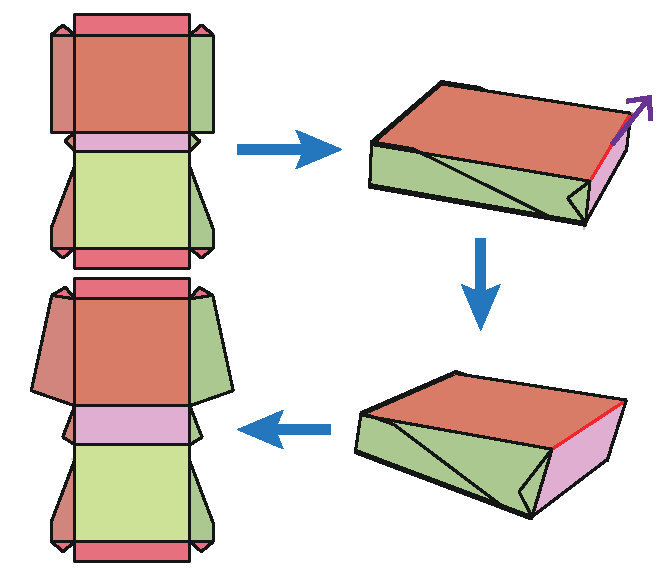
\includegraphics[width=0.36\textwidth]{images/editing1}
		\label{fig:editing1}
	}
	\hspace{4ex}
	\subfigure[]{
		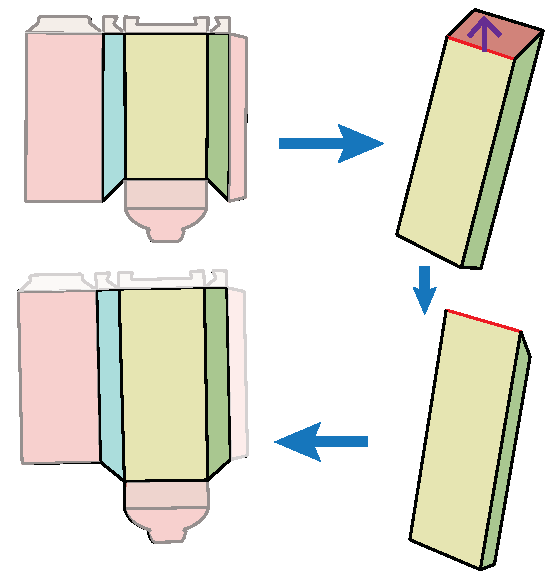
\includegraphics[width=0.3\textwidth]{images/editing2}
		\label{fig:editing2}
	}
	\caption{Two examples of layout modification from 3D model editing. For each example, a box-like carton can be generated from the given 2D layout. Users can edit the shape of the 3D carton by dragging edges in our system. By enforcing the shape rigidity constraints, our system automatically updates the 2D layout.}
	\label{fig:editing}
\end{figure}
 
\paragraph{Panel pasting.} Merging vertexes is sometimes not enough to generate a desired model because of glue flaps, as shown in Figure~\ref{fig:facepasting}. 
%
Many small flaps should be pasted to their adjacent side panels when making a carton; therefore, our system automatically detects panels to paste together. 
A pair of panels $P_a$ and $P_b$ is considered mergeable if their normals, $\mathbf{n}_a$ and $\mathbf{n}_b$, satisfy $\mathbf{n}_a \cdot \mathbf{n}_b > 0.5$, and for each vertex in $\{\mathbf{v}^{a}_{i}\}_{i=1}^{N_a}$ of the panel $P_a$,  $|(\mathbf{v}^{a}_{i} - \mathbf{v}_{c}^b) \cdot \mathbf{n}_b| < \epsilon_d$, where $\mathbf{v}_{c}^b$ is the centroid of the panel $P_b$, and $\mathbf{n}_b$ is its normal. When involving multiple panels, the detection strategy is the same as the vertex merging step. 



\subsection{2D Layout Refinement from 3D Editing}
Our system is highly efficient for generating a 3D carton from an existing 2D layout. It also 
allows users to creatively edit the current 3D carton model by dragging an edge, and it simultaneously refines the 2D layout automatically according to the 3D editing.
%
When the 3D mesh changes, the new shape constraints are transferred to the 2D layouts by maintaining the panel rigidity (Eq.~\ref{equ:plane}).
Since the layout remains in a 2D plane, the coplanarity is enforced by set all the vertexes in the layout to lie on the $XoY$ plane.  
% 
The irrelevant vertexes that do not lie on the moving edge have to stay at their original locations, as described in Eq.~\ref{equ:irrelevant}.
Figure~\ref{fig:editing} shows two examples of automatic refinement of 2D layouts based on 3D editing.                                                                     


